\subsection{Modelagem do PA}

Para fazer a modelagem em software foi utilizada a linguagem de programação Python. Para isso, separou-se os dados citados na seção \ref{sec:implsoft}, em dados de extração e dados de validação, os quais são utilizados para extração dos coeficientes do modelo do MP e validação do modelo encontrado, respectivamente. Para fazer a validação do modelo utilizou-se a métrica do NMSE, que consiste em calcular o erro quadrático médio do valor medido pelo VSA (Analisador de Sinal Vetorial) para o valor calculado pelo modelo. Portanto, quanto menor o NMSE mais fiel é o modelo do PA. Nesta etapa obteve-se um NMSE de -23.57 dB, para cálculos em vírgula flutuante, onde o resultado está presente no gráfico da figura \ref{fig:modelopafloat}.

\begin{figure}[htbp]
    \centering
    \captionsetup{justification=centering}
    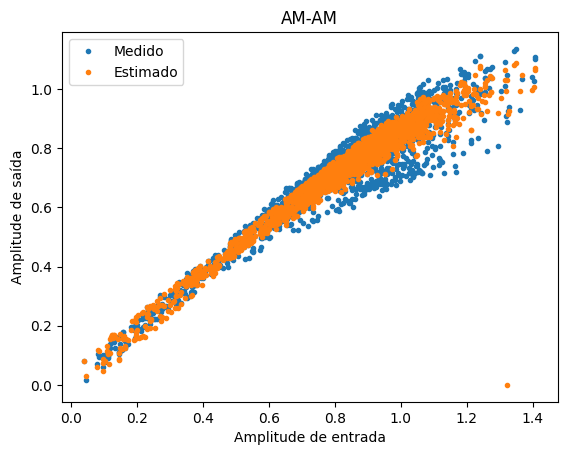
\includegraphics[width=\figsize]{modeloPAfloat.png}
    \caption{Modelo do PA em vírgula flutuante}
    \label{fig:modelopafloat}
\end{figure}

\subsection{Definição do número de bits}

Após concluída a modelagem matemática, realizou-se a modelagem do PA para então ser feito o levantamento da quantidade de bits necessários para a implementação do DPD em hardware minimizando os erros de quantização. 
Para isso foi necessário refazer a extração dos coeficientes, mas desta vez com os dados normalizados para valores de 0 a $2^{bits}$.  
O resultado desse levantamento está presente no gráfico na figura \ref{fig:bits}.

\begin{figure}[htbp]
    \centering
    \captionsetup{justification=centering}
    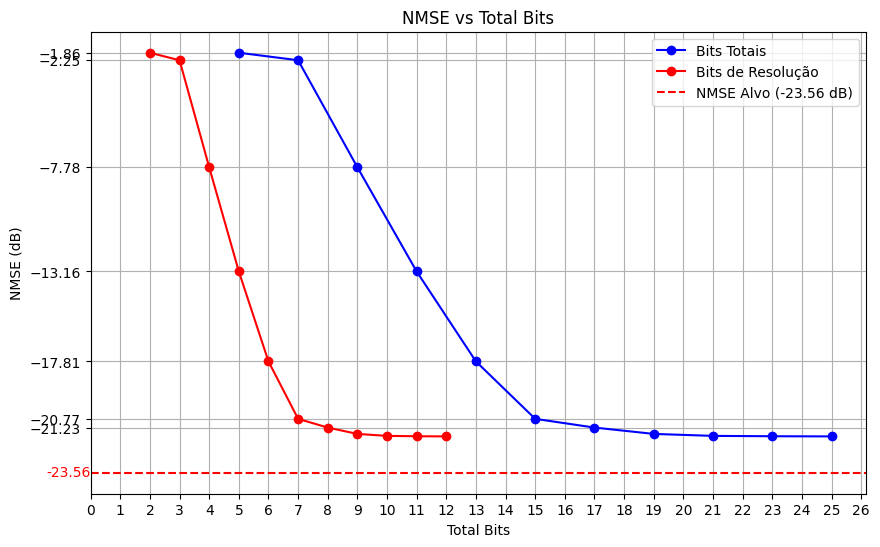
\includegraphics[width=\figsize]{bits.png}
    \caption{Gráfico Número de bits x NMSE}
    \label{fig:bits}
\end{figure}

Neste gráfico observa-se duas curvas, a curva em azul apresenta a quantidade total de bits contando com os bits de overflow necessárias para as operações de multiplicação, enquanto a curva em vermelho representa a quantidade de bits de resolução do sinal. Analisando este gráfico observou-se que não existem ganhos significativos no erro a partir de 8 bits, portanto foi feita a modelagem do PA utilizando uma resolução de 8 bits. O resultado alcançado está ilustrado pela figura \ref{fig:modelopa}.

\begin{figure}[htbp]
    \centering
    \captionsetup{justification=centering}
    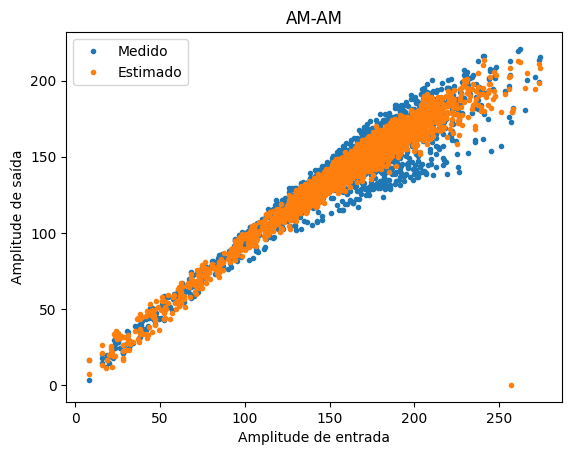
\includegraphics[width=\figsize]{modeloPA.png}
    \caption{Modelo do PA em vírgula fixa}
    \label{fig:modelopa}
\end{figure}

\subsection{Modelagem do DPD}
A partir dos resultados obtidos foi possível fazer a modelagem do DPD, para isso foi feito o mesmo processo de modelagem do PA, porém para alcançar a característica de transferência inversa do PA foi invertido a ordem dos dados de entrada e saída para extração dos coeficientes do DPD. O resultado desta modelagem está ilustrado pela figura \ref{fig:modelodpd} a seguir.

\begin{figure}[htbp]
    \centering
    \captionsetup{justification=centering}
    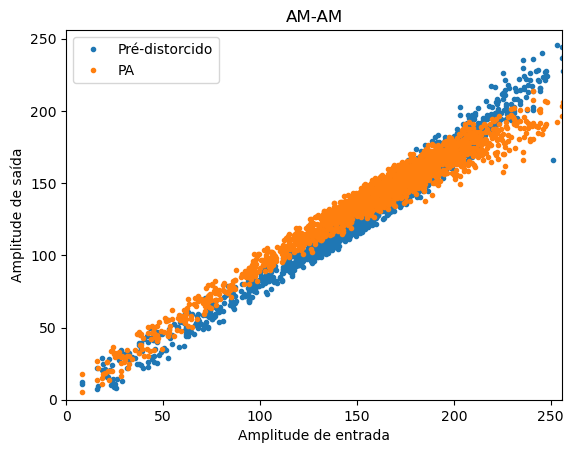
\includegraphics[width=\figsize]{modelodpd.png}
    \caption{Modelo do DPD em vírgula fixa}
    \label{fig:modelodpd}
\end{figure}

\subsection{Implementação do DPD em FPGA}

E por fim foi implementado o código em VHDL para FPGA.
Para que essa arquitetura de hardware apresentasse uma boa performance, todas as operações aritméticas (soma e multiplicação) são realizadas de forma síncrona. Então foi necessário dividir cada uma em processos distintos. A saída de um processo alimenta um \textit{buffer}, que serve como entrada para o próximo processo. A Figura \ref{fig:diagramaprocesssimpl} ilustra essa arquitetura de maneira simplificada.

\begin{figure}[htbp]
	\centering
	\captionsetup{justification=centering}
	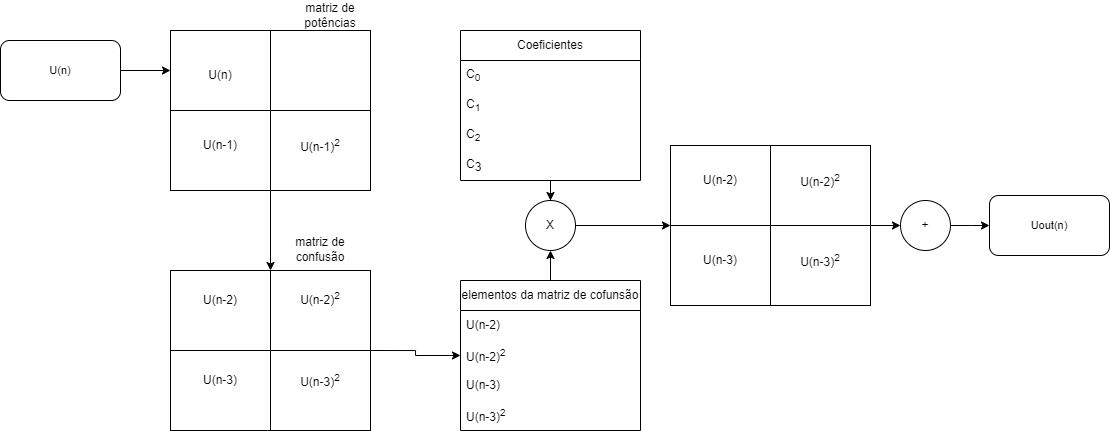
\includegraphics[width=\figsize]{processo_simplificado.png}
	\caption{Processo de cálculo da saída}
	\label{fig:diagramaprocesssimpl}
\end{figure}

O resultado dessa implementação foi simulado em uma FPGA Virtex5 XC5VLX50T, utilizando um total de 150 registradores, 692 LUTs e 4 DSP48Es, operando a uma frequência de 61,44 MHz. A Figura \ref{fig:fpgasim} apresenta o resultado dessa implementação, representado pelos "x" em vermelho, em comparação com o resultado da simulação em Python, indicado pelos "°" em azul.

\begin{figure}[htbp]
	\centering
	\captionsetup{justification=centering}
	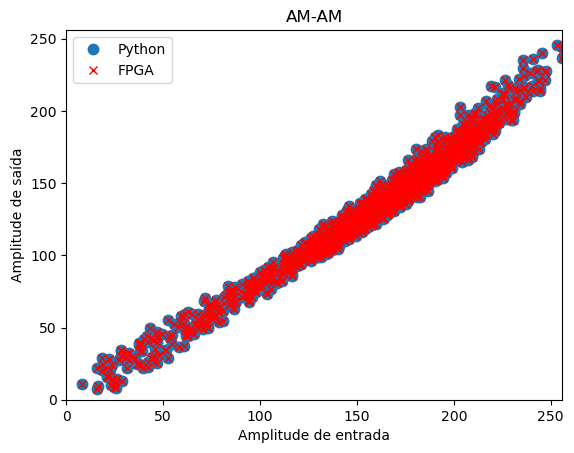
\includegraphics[width=\figsize]{fpgasim.png}
	\caption{Processo de cálculo da saída}
	\label{fig:fpgasim}
\end{figure}
